\documentclass[conference]{IEEEtran}
\usepackage{graphicx}
\usepackage{fixltx2e}
%\usepackage{mathtools}
\usepackage[cmex10]{amsmath}
\usepackage[cmex10]{amsmath,mathtools}

%header info
\usepackage{fancyhdr}
\pagestyle{fancy}
\lhead{Griffith University - School of Engineering}
\rhead{page \thepage}

%table manipulation
\usepackage{supertabular,booktabs,tabularx}
\newcolumntype{C}{>{\centering\arraybackslash}X} % centered version of "X" type

%for subfigures - side by side figures
\usepackage{caption}
\usepackage{subcaption}

%wrapped figures
\usepackage{wrapfig}





% *** MATH PACKAGES ***
%
\usepackage[cmex10]{amsmath}


% correct bad hyphenation here
\hyphenation{op-tical net-works semi-conduc-tor}


\begin{document}

%
% paper title
% can use linebreaks \\ within to get better formatting as desired
% Do not put math or special symbols in the title.
\title{Colour Analysis of Strawberries on a Real Time Production Line}



%%%%%%%%%%%%%%%%%%%%%%%%%%%%%%%%%%%%%%%%%%%%%%%%%%%%%%%%%%%%%%%%%%%%%%

\author{\IEEEauthorblockN{Gilbert Eaton\IEEEauthorrefmark{1},
		Andrew Busch\IEEEauthorrefmark{2}, Rudi Bartels\IEEEauthorrefmark{3} and
		Yongsheng Gao\IEEEauthorrefmark{4}}
\IEEEauthorblockA{Griffith School of Engineering\\
Griffith University, Nathan
Brisbane, Queensland 4122\\
Sept 2018}

Email: \IEEEauthorrefmark{1}gilbert.eaton@griffithuni.edu.au,
\IEEEauthorrefmark{2}a.busch@griffith.edu.au,
\IEEEauthorrefmark{3}r.bartels@griffith.edu.au,
\IEEEauthorrefmark{4}yongsheng.gao@griffith.edu.au}



% make the title area
\maketitle

% As a general rule, do not put math, special symbols or citations
% in the abstract

%%%%%%%%%%%%%%%%%%%%%%%%%%%%%%%%%%%%%%%%%%%%%%%%%%%%%%%%%%%%%%%%%%%%%%%%%%
\begin{abstract}


A novel system has been designed where colour analysis algorithms facilitate grading ripeness of packed strawberries on a fast-paced production line. The Strawberry quality system acquires images at the rate of $2 punnets/s$, and feeds the images to the two algorithms. Using CIELAB and HSV colourspaces, both underripe and overripe colour features are analysed  resulting in F1 scores of $94.7\%$ and $90.6\%$ respectively, when measured on multiple defect samples. The single defect class results scored $80.1\%$ and $77.1\%$. The algorithms total time for the current hardware configuration is $121ms$ maximum and $80ms$ average, which is well below the required time window of $500ms$.

$105,542$ punnets have been assessed by the algorithm and has rejected $4,952$ in total ($4.9\%$),  helping to ensure the quality of the product being shipped to customers and avoiding costly returns.


\end{abstract}

%%%%%%%%%%%%%%%%%%%%%%%%%%%%%%%%%%%%%%%




%%%%%%%%%%%%%%%%%%%%%%%%%%%%%%%%%%%%%%%%%%%%%%%%%%%%%%%%%%%%%%%%%%%%%%%%%%

\IEEEpeerreviewmaketitle

\section{Introduction}
% no \IEEEPARstart

Real-time colour grading is an essential part of quality assessment of fruits and vegetables in order to determine ripeness or consistency, and can be used to detect skin blemishes caused by rots, mould, pests, or mishandling \cite{blasco}. Historically, this has been performed by the people harvesting and packing them, however, the industry has recently been utilizing new technologies instead of relying on manual intervention for sorting/grading produce \cite{londhe}. Automating these processes can be very difficult to achive in agriculture, particularly in fast-paced environments where tons of produce flows from field and through to the supply chain for consumers daily. Modern advances in both computers and vision systems have allowed this type of analisis to be integrated in many production/packing lines around the world. Discussed in this article, the colour analysis method used by our vision system on a commercial strawberry packing line.

Colour analysis is commonly used as an indication of the quality of fruits and vegetables, where these features can be used to grade/sort items into categories \cite{jun, elmasry}, to detect skin blemishes \cite{blasco, leemans}, size and volume estimation \cite{bundit, elmasry}, and texture analysis \cite{jun, rakuna}. Multiple cameras have been used (often requiring multiple processors) to minimise uninspected surfaces \cite{zouxiou, quingzong}, to assess multiple defects \cite{blasko2}, counting \cite{song}, 3D reconstruction \cite{panitat} or to allow speed increases\cite{recce}.   

Other methods for fruit and vegetable quality analysis have been adopted such as infra-red image analysis or spectroscopy \cite{guthrie, bureau, yande}, and hyperspectral imaging \cite{renfu} \cite{jianwei, mendoza, rajkumar}. These acquisition systems can be used to detect defects such as internal structure estimation, soluable solids content, under-skin defects and pests, and maturity. Utilizing different wavelengths, it is a common approach to find a suitable spectral position to observe the best contrast for defects, making these features easier to extract\cite{ariana, piotr}. The system under development is intended to use a combination of colour (RGB) and infra-red (IR) bands in the future, to assess specific types of reject class such as brusing and potentially pest infestation. 

Using a conveyor system, L. Xu et al \cite{xu} achieved very good results in classifying shape, ripeness, and size of strawberries. The measurements are attained by using a K-means clustering method to find 7 vertical and 7 horizontal axis lines. Size feature was calculated by performing experiments to find the ratio of pixels/mm and simply dividing the pixel measurements of the berry by this ratio. Using the CIELAB colour space, a dominant colour was found in the berry by means of a histogram windowing method. Liming et al \cite{liming} used a similar approach to grade single strawberries on a conveyor in real-time. They extracted shape features by using normalised line segments on the contour with a K-means clustering method to evaluate the shape, size features by experimentally attaining the camera-object distances in terms of mm/pixel, and colour features using a CIELAB a-channel histogram windowing method to find the dominant red colour. The CIELAB colour space was also used by Lin et al \cite{lin} when they developed a strawberry calyx removal system. The single strawberries entered the vision enclosure on roller rods, before being analysed using image processing to find orientation, and finally a high pressure water jet was used to cut the green parts of the strawberry off and discarding.


The strawberry field-harvesting robot commissioned by Hayashi et al \cite{hayashi} within a greenhouse, used a method of calculating the 'Maturity Level' by analysing specific bands of the HSI colour space which represented ripe and underripe colours and intensities. As it was determined that the strawberries would be either underripe or ripe, with the event of over-ripeness ignored due to the constant operation of the harvester. They chose values of H,S, and I that equated to the colours red for ripe, whilst green, light pink, and dark pink were used for underripe in order to evaluate the ripeness before the robot picked the berries. Satoshi et al \cite{satoshi} also developed a robot harvester which used a red LED, green LED, and white LED to illuminate the scene in different colours before acquiring images with the same camera in order to best extract the subtle differences in shades of red and pink on the berries. 

All methods researched involved imaging single strawberries, either stationary or moving on a slow conveyor. This assumption is both inefficient and impractical given the high throughput of packing facilities and delicate flesh of the strawberry.

The proposed system in this article will perform quality grading of all fruits after they are packed in a real-time, fast-paced environment. This unique and novel vision system is designed to be capable of efficient and accurate in-line quality control for a large agricultural business.   

 
%%%%%%%%%%%%%%%%%%%%%%%%%%%%%%%%%%%%%%%



%%%%%%%%%%%%%%%%%%%%%%%%%%%%%%%%%%%%%%%%%%%%%%%%%%%%%%%%%%%%%%%%%%%%%%%%%%
%\newpage
\section{Materials and Methods}
 

The enclosure has been designed to have a robust structure, due its placement on the production floor, and is equipped with safety systems, signals, and controls for operator use. The shell is made from $5mm$ stainless steel sheeting bolted to a $40mm$ aluminium frame. The enclosure houses all electronics, hardware and software required for sensing punnets, acquisition, and controlling the system.




\subsection{Image Acquisition} 


The system encloses part of the production line for lighting control, using DC power and cross polarizers to stabilize the intensity \cite{eaton}. In order to capture the punnets without motion blur, the shutter speeds of the cameras must be less than $3ms$ due to the production line speed of $16.6m/min$ ($0.276m/s$). Given this shutter speed restriction, along with the added diffusers and cross-polarizers, the total illumination power required is $1200W$. Figure \ref{fig:enclosure_cross_sec} shows a CAD drawing of the enclosure, lighting and diffuser positions, the camera set up above and below the v-belt conveyor, and the computer/electronic componet section underneath the conveyor.

\begin{figure}[ht]
	\centering
	\begin{subfigure}{.5\textwidth}
		\centering
		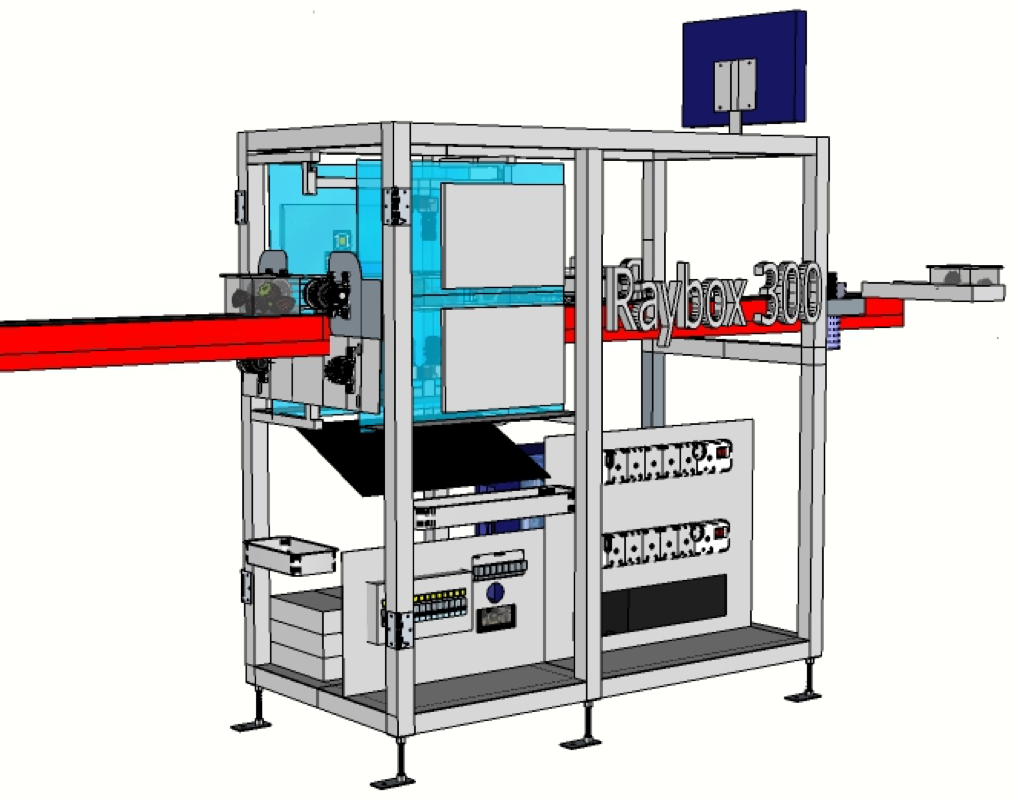
\includegraphics[width=1\linewidth]{eps/SQA_v2.eps}
		\caption{}
		\label{fig:enclosure_cross_sec}
	\end{subfigure}%
	
	\vspace{\floatsep}
	
	\begin{subfigure}{.5\textwidth}
		\centering
		\includegraphics[width=1\linewidth]{eps/QAS_cross_sec.eps}
		\caption{}
		\label{fig:close_up_cross_sec}
	\end{subfigure}%
	
	\caption{Top: Components of the full system - conveyors, diffusers and polarisers, as well as electronic/computer storage. Bottom: Close up of the v-belt conveyor system and the camera set up. }
	\label{fig:sample1}
\end{figure}

The colour (BFLY-U3-23S6C-C) and mono (BFLY-U3-23S6M-C) cameras are both manufactured by Point Grey (Flir Integrated Imaging Solutions, Inc.) using the Sony IMX249 sensor with a resolution of 1920x1200 and USB3 interface. As the Quantum Efficiancy (QE) is much higher on the mono camera, it is used for NIR imaging due to the higher responses at these wavelengths.

The computer is a standard desktop PC with an ASUS P8Z68 motherboard and an 8-core i7 CPU. An Advantec PCE-USB4-00A1E four port dedicated USB3 PCI-e card is installed to ensure bandwidth is sufficient for all of the cameras. The enclosure, in Figure \ref{fig:enclosure_front}, shows the front view of the system with control panel and display, as well as the punnet conveyor infeed and outfeed. 

\begin{figure}[h]
	\centering
	\includegraphics[scale=0.05]{eps/enclosure_front.eps}
	\caption{Lighting enclosure showing control panel and punnet conveyor}
	\label{fig:enclosure_front}
\end{figure}


As each punnet enters the enclosure, it is detected by a photoelectric sensor which triggers the acquisition sequence. The $100W$ LED chips generate large amounts of heat due to the compact array of 100-$1W$ individual LED's. Therefore, thermal control is required to keep the LED chips from overheating. A combination of strategies has been integrated such as using $5mm$ thick stainless steel plates for heat dissipation (sink), thermal compound between LED and heatsink, and strobing the LED to reduce the duty cycle and allow cooling between images.   



\subsection{Colour Analysis}
\label{sec:colour_analysis}

The colour analysis (and all other accompanying analyses) performed must execute and complete within $500ms$ in order to assess each and every punnet. As each image is processed by up to 10 algorithms, the runtime duration of each must be reduced where possible. Although machine learning strategies such as SVM and nueral networks may improve accuracy, initial experiments showed that these classifiers require large datasets that are well labelled to perform adequate training. The time complexity of neural networks also poses a problem due to the restricted processing time \cite{he}\cite{angiulli}. 

The colour analysis described in this paper is used to distinguish under ripe and over ripe punnets. Each punnet is processed as a discrete unit, as single berries cannot be physically removed, therefore the punnet is assessed as either pass or fail in totality, with the reject berries to be replaced after inspection. This corresponds to the customer quality performance reports which indicate number of punnets rejected as opposed to number of berries. 

Market conditions, weather, supply chain, and seasonality can greatly affect the quality of crops in general, but particularly for strawberries as they are not considered a hardy fruit unlike apples and oranges. As these adversarial factors occur, the impact seen on the strawberry market can change dramatically from pricing and quality to short supply. The packing operators must be able to account for these dynamic conditions by increasing and decreasing the acceptable standard. This means that under certain circumstances, underripe, overripe, misshapen or even fruit usually considered to be too small will be packed and shipped due to market availability. Given this variation of requirements by the operators, the system must have the ability to adjust the thresholds of each quality characteristic, and therefore only reject punnets based on current market conditions or recent weather. 

In order to overcome speed concerns, and to reduce overall processing time, the colour algorithm is designed to scale each image down from a high resolution to a fraction of the original, and assess regions comprised of less pixels. This direction is, again aligned with the customer expectations due the inherrant fact that very small regions ($<3mm$) will be largely ignored by visual inspections. It is only the larger, connected regions which determine overall ripeness.

The saturation channel of the $HSV$ colourspace is used initially find the berries in each frame, due to the more colourful berries and punnet when compared to the dark background. 

To extract HSV colourspace given three channels R, G, B and $Min = min(R, G, B)$, $Max = max(R, G, B)$:
\begin{equation}
H = 
\begin{cases} 
rad(60) \times \frac{(G-B)}{Max-Min}, & R=Max \\
rad(60) \times \frac{(B-R)}{Max-Min} + 2, & G=Max \\
rad(60) \times \frac{(R-G)}{Max-Min} + 4, & B=Max \\   
\end{cases}
\end{equation}
\begin{equation}
S = 
\begin{cases} 
0, & Max=Min \\   
(Max-Min)/Max, & otherwise        
\end{cases}
\end{equation}
\begin{equation}
V = Max
\end{equation}


However, as the colour white has low saturation and can appear on underripe berries, this must be identified, extracted and concatenated to the region in order to properly calculate the underripe region areas. The red berry and white berry usually converge gradually so that the regions overlap when extracted. This means that simply taking the intersection of all white regions with known red berry regions will yield only those which are overlapping red berry as described in equations \ref{red_berry_thresh}, \ref{white_berry_thresh}, and \ref{intersect_white_berry}.

\begin{equation}
	R_{red} = \sum_{i=0}^{P}t1<S_i<max(S)
	\label{red_berry_thresh}
\end{equation}

\begin{equation}
	R_{white} = \sum_{i=0}^{P}t2<V_i<max(V)
	\label{white_berry_thresh}
\end{equation}

\begin{equation}
	R_{overlap} = R_{white} \cap R_{red}
	\label{intersect_white_berry}
\end{equation}

where the red and white regions ($R$) are found by using threshold values $t1$ and $t2$ over the number of pixels $P$, on the saturation ($S$) and value ($V$) channels of the transformed image, respectively. If $R_{overlap}$ is greater than zero, then $R_{white}$ is concatenated with the known red regions. 
 

\begin{figure}[h]
	\centering
	\includegraphics[scale=0.35]{eps/CIELab-colour-space.eps}
	\caption{CIELAB colourspace}
	\label{fig:lab}
\end{figure}


The $CIELAB$ colourspace axes values fit this colour analysis problem well, in that the $a^*$ channel axis contains red and green hues, and the $b^*$ channel blue and yellow (fig \ref{fig:lab}). 

Strawberries are member of the nonclimacteric class of fruit, meaning that ripening halts once harvested. Strawberries are more firm and will transport better when harvested just before full ripeness, although are not as full in flavour as entirely ripened fruit\cite{artur}, therefore it is acceptable for customers and realistic for pickers to expect some amount of underripeness as well as overripeness.

\subsubsection{Underripe Features}

The ripening process, in terms of colour, for most fruit will start green and slowly transition through phases of yellow/orange, then pink before bright red and finally dark red. Figure \ref{fig:yellow_white} shows an image containing underripe berries, the yellow and white regions clearly seen.

Once the berry contour has been found and the image domain reduced to that region, underripe pixels are extracted by simply taking the difference of the $a^*$ channel and the $b^*$ channel. After contrast enhancement, areas with no red pixels are highlighted. The process is visualised in Figure \ref{fig:underripe_process}. Perfoming this analysis on the entire image results in many false positives, but this method has been found to be very effective when applied to the known berry region.   

\begin{figure}[ht]
	\centering
	\begin{subfigure}{.25\textwidth}
		\centering
		\includegraphics[width=.9\linewidth]{eps/zoom_image.eps}
		\caption{}
		\label{fig:yellow_white}
	\end{subfigure}%
	\begin{subfigure}{.25\textwidth}
		\centering
		\includegraphics[width=.9\linewidth]{eps/hsv_contour.eps}
		\caption{}
		\label{fig:hsv}
	\end{subfigure}%
	
	\begin{subfigure}{.25\textwidth}
		\centering
		\includegraphics[width=.9\linewidth]{eps/pow_image.eps}
		\caption{}
		\label{fig:pow_image}
	\end{subfigure}%
	\begin{subfigure}{.25\textwidth}
		\centering
		\includegraphics[width=.9\linewidth]{eps/result.eps}
		\caption{}
		\label{fig:result}
	\end{subfigure}%
	
	\caption{Left to right: (a)Original image with visible white and yellow regions, (b)HSV saturation channel and berry contours after addition of white berry regions, (c)Diff(a*, b*) result highlighting absence of red colour, (d)Result of post-processing indicating underripe areas.}
	\label{fig:underripe_process}
\end{figure}


\subsubsection{Overripe Features}

\begin{figure}[ht]
	\centering
	\begin{subfigure}{.25\textwidth}
		\centering
		\includegraphics[width=.9\linewidth]{eps/over_berries.eps}
		\caption{}
		\label{fig:over_berries}
	\end{subfigure}%
	\begin{subfigure}{.25\textwidth}
		\centering
		\includegraphics[width=.9\linewidth]{eps/over_hue.eps}
		\caption{}
		\label{fig:over_hue}
	\end{subfigure}%
	
	\begin{subfigure}{.25\textwidth}
		\centering
		\includegraphics[width=.9\linewidth]{eps/over_diff_hue.eps}
		\caption{}
		\label{fig:over_diff}
	\end{subfigure}%
	\begin{subfigure}{.25\textwidth}
		\centering
		
\includegraphics[width=.9\linewidth]{eps/over_light.eps}
		\caption{}
		\label{fig:over_light}
	\end{subfigure}%
	
	\begin{subfigure}{.25\textwidth}
		\centering
		
\includegraphics[width=.9\linewidth]{eps/over_light_diff.eps}
		\caption{}
		\label{fig:over_light_diff}
	\end{subfigure}%
	\begin{subfigure}{.25\textwidth}
		\centering
		\includegraphics[width=.9\linewidth]{eps/over_result.eps}
		\caption{}
		\label{fig:over_result}
	\end{subfigure}%
	
	\caption{Left to right: (a)Berry region extracted using method from underripe algorithm, (b)Result of thresholding expanded HSV hue channel to find light colour berries, (c)Difference region of $a$ and $b$, (d)V channel used to illiminate edges. e)Intersection result of $c$ and $d$, (f)Overripe berries extracted.}
	\label{fig:overripe_process}
\end{figure} 

The colour difference between ripe and overripe berry is much narrower than the comparrison with underripe. Underripe colours may be white, green, yellow, or pink whereas overripe colour is a slightly darker red than perfectly ripened berries appear. This small variation combined with the many occlusions make the overripe features difficult to extract.

Shadowy areas of the punnet can be falsely classified as overripe berry, as the colour profiles are very similar. Therefore, the algorithm must exclude the edges of the berries in order to improve the accuracy of identifying overripe features. 

\begin{table*}
	\caption{Results of algorithm testing.}
	\label{tab:algo_test}
	\begin{tabularx}{\textwidth}{@{}l*{8}{C}c@{}}
		\toprule
		Algorithm & Defects & FP  & FN  & TP  & TN  & Precision(\%) & Recall(\%) & F1 score(\%) & Y-Index(\%)\\ 
		\midrule
		Underripe   & Single   & 19 & 90 & 220 & 198 & 92.1 & 71.0 & 80.1 & 62.2 \\[6pt] 
		& Multiple & 7  & 25 & 285 & 210 & 97.6 & 91.9 & 94.7 & 88.7 \\[6pt]
		Overripe    & Single   & 44 & 82 & 212 & 177 & 82.8 & 72.1 & 77.1 & 52.2 \\[6pt]
		& Multiple & 19 & 35 & 259 & 202 & 93.2 & 88.1 & 90.6 & 79.5 \\[6pt]	 
		\bottomrule
	\end{tabularx}
\end{table*}

Using a known vector range in the $HSV$ colourspace $\{H_0, S_0, V_0\}, \{H_1, S_1, V_1\},....,\{H_n, S_n, V_n\}$, the good quality berry colour is  extracted and compared to the entire berry region as shown in Figure \ref{fig:over_berries}, \ref{fig:over_hue} and \ref{fig:over_diff}. Note that if there is sufficient underripe regions the algorithm will end before this point. Therfore, the vector range is inclusive of underripe colours ensuring only darker pixels are extracted in the difference of the two regions.


In order solve the problem of berry edges, an intensity threshold is applied which ignores the darker areas of the punnet including voids, berries too dark to grade, and edges where shadows occur (Fig. \ref{fig:over_light}). Performing an intersection of these regions with the dark pixels found ensures that any overripe candidate must lie on the un-occluded surfaces of berries in order to be classified properly. 
\begin{equation}
R_{cand} = R_{berry} - R_{good}
\label{diff_berry_hue}
\end{equation}

\begin{equation}
R_{norm} = \sum_{i=0}^{P}t3<V_i<max(V)
\label{berry_tops}
\end{equation}

\begin{equation}
R_{overripe} = R_{cand} \cap R_{norm}
\label{intersect_dark_berry}
\end{equation}

$R_{cand}$ is the candidate overripe region which may still contain false-positive pixels. The threshold to find the surface normal ($R_{norm}$) of the berries is then intersected with the candidates to highlight only confident matches as shown in Figures \ref{fig:over_light_diff} and \ref{fig:over_result}.


%%%%%%%%%%%%%%%%%%%%%%%%%%%%%%%%%%



%%%%%%%%%%%%%%%%%%%%%%%%%%%%%%%%%%%%%%%%%%%%%%%%%%%%%%%%%%%%%%%%%%%%%%%%

\section{Application and results}


The colour analysis algorithms have been implemented on the production line and, at the date of this paper, graded 105,542 punnets of which 4952 punnets were rejected due to failing to meet colour requirements. Continuous grading on-line will ensure that the quality of the product being packed will meet the customer requirements, and prevent reject shipments. Reject shipments can occur even when just a few poor quality punnets are observed forcing costly returns, loss of product, and reduced reputation in the industry.


Both algorithms have input sensitivity levels to help deal with seasonality. As discussed in section \ref{sec:colour_analysis}, the seasonality determines the acceptability of the fruit. This allows operators to, for example, change the sensitivity and allow slightly poorer quality fruit to pass, whilst still maintaining a threshold to remove moderate and severe cases.

Due to this variability in reject level, the quantitative analysis was split into two different measurements - single defect and multiple defects. Multiple defects meaning that there exist more than one region of the same reject class in each image. For example, a multiple defect underripe punnet will have greater than one region (that meets certain conditions) with underripe features.

Table \ref{tab:algo_test} lists the results of testing for both algorithms where the test set was ground truthed with 310 out of 527 punnets underripe, and 294 out of 515 punnets overripe in a separate set. In order to best compare the single and multiple defect classes, the same test punnets were used with the addition of more defect fruit for the multi-defect instances. The confusion matrices for the tests are detailed in tables \ref{tab:confusion_1},  \ref{tab:confusion_2}, \ref{tab:confusion_3} and \ref{tab:confusion_4}.

\begin{table}
	\centering
	\caption{Confusion matrix for single defect underripe tests.}
	\label{tab:confusion_1}
	\begin{tabular}{ccc}
		\toprule
		$n=527$ & Predicted: Good & Predicted: U/R  \\ 
		\midrule
		Actual: Good   & 198 & 19    \\[6pt] 
		Actual: U/R	   & 90  & 220  \\[6pt] 
		\bottomrule
	\end{tabular}
\end{table}

\begin{table}
	\centering
	\caption{Confusion matrix for multiple defect underripe tests.}
	\label{tab:confusion_2}
	\begin{tabular}{ccc}
		\toprule
		$n=527$ & Predicted: Good & Predicted: U/R  \\ 
		\midrule
		Actual: Good   & 210 & 7    \\[6pt] 
		Actual: U/R	   & 25  & 285  \\[6pt] 
		\bottomrule
	\end{tabular}
\end{table}

\begin{table}
	\centering
	\caption{Confusion matrix for single defect overripe tests.}
	\label{tab:confusion_3}
	\begin{tabular}{ccc}
		\toprule
		$n=515$ & Predicted: Good & Predicted: O/R  \\ 
		\midrule
		Actual: Good   & 177 & 44    \\[6pt] 
		Actual: O/R	   & 82  & 212  \\[6pt] 
		\bottomrule
	\end{tabular}
\end{table}

\begin{table}
	\centering
	\caption{Confusion matrix for multiple defect overripe tests.}
	\label{tab:confusion_4}
	\begin{tabular}{ccc}
		\toprule
		$n=515$ & Predicted: Good & Predicted: O/R  \\ 
		\midrule
		Actual: Good   & 202 & 19    \\[6pt] 
		Actual: O/R	   & 35  & 259  \\[6pt] 
		\bottomrule
	\end{tabular}
\end{table}


The number of punnets for each test is broken into false positive, false negative, true positive, and false negative, used to calculate precision, recall, and F1-score as well as Youden's index or J statistic. Youden's index (Y-Index) is the measure of the performance of a dichotomous diagnostic test where informedness is the generalization of this method to a multi-class set.

F1-Score results for multiple defects are calculated as $94.7\%$ and $90.6\%$ for the underripe and overripe algorithms respectively. The single defect class results scored $80.1\%$ and $77.1\%$ given the high probability of occlusion and shadows, and rotational variance of each berry.

Recall takes the ratio of the relevant class selected over the entire relevant class. For example, how many underripe detections were made compared to the total amount of underripe punnets. Precision measures the amount of correct detections compared to all detections. 

This indicates for both the underripe and overripe results the flase negatives are greater than the false positives. This was an intentional bias in development in order to gain maximum acceptance from operators and managers at the facility. If the system was to have low precision (even with high recall), it may be seen as more of a burden than a benifit to smooth operation of the packing line.

The total propogation time of both algorithms had a maximum of $121ms$ and average of $80ms$ when tested on a series of 100 images. The processing window is $500ms$ (time between punnets at max speed) and therefore computes and makes a decision within the required timeframe.

%%%%%%%%%%%%%%%%%%%%%%%%%%%%%%%%%%%


%%%%%%%%%%%%%%%%%%%%%%%%%%%%%%%%%%%%%%%%%%%%%%%%%%%%%%%%%%%%%%%%%%%%%%%%

\section{Conclusion}

Two colour analysis algorithms were developed to assist in grading packed strawberries in a real-time production environment. Multiple defect detection results indicate the validity of the system and it's accuracy, and operators can tune the system to suit the market conditions. However, further work is required in order to detect single defect cases more accurately. 

The inspection system, along with these algorithms have already helped in reducing the amount of poor quality berries being shipped by the company, leading to increased Quality Assurance, Quaity Control, and mitigating potential financial losses.


\subsection{Future Work}


With images being acquired daily from the production line, labelling can begin in order to provide a large enough dataset to enable deep learning strategies. For example, an SVM classifier could be trained with a few hundred labelled images, but tens of thousands would be required for training a neural network which is the ultimate goal. 



   

%%%%%%%%%%%%%%%%%%%%%%%%%%%%%%%%%%%





% use section* for acknowledgement
\section*{Acknowledgment}

The authors would like to acknowledge the ARC linkage program as well as Magnificent Pty. Ltd for their ongoing support of this project. 



\bibliographystyle{ieeetr}


\begin{thebibliography}{1}
	
	%1
	\bibitem{blasco}
	J. Blasco, N.Aleixos, E.Moltó, ``Machine Vision System for Automatic Quality Grading of Fruit,'' {\em Biosystems Engineering}, Vol: 85(4) (2003) pp 415-423.
	
	%2
	\bibitem{londhe}
	Dattatraya Hiraman Londhe, Sachin Madhukar Nalawade, Ganesh Shyamrao Pawar, Vinod Tukaram Atkari, Sachin Vilas Wandkar, ``Grader: A review of different methods of grading for fruits and vegetables'' {\em Agric Eng Int: CIGR Journal}, Vol: 15 No.3 (2013) pp 217-230.
	
	%3
	\bibitem{jun}
	Jun Zhao, J. Tow, J. Katupitiya, ``On-tree Fruit Recognition
	Using Texture Properties and Color Data,'' {\em Intelligent Robots and Systems}, DOI: 10.1109/IROS.2005.1545592 (2005).
	
	%4
	\bibitem{elmasry}
	Gamal El Masry,  Sergio Cubero,  Enrique Moltó,  José Blasco, ``In-line sorting of irregular potatoes by using automated computer-based machine vision system,'' {\em Journal of Food Engineering}, Vol: 112 (2012) pp 60-68.

	%5
	\bibitem{leemans}
	V. Leemans, Hugo Magein, M. F. Destain, ``On-line Fruit Grading according to their External Quality using Machine Vision,'' {\em Biosystems Engineering}, Vol: 83(4) (2002) pp 397-404.
	
	%6
	\bibitem{bundit}
	Bundit Jarimopas, Nitipong Jaisin, ``An experimental machine vision system for sorting sweet tamarind,'' {\em Journal of Food Engineering}, Vol: 89 (2008) pp  291-297.
	
	%7
	\bibitem{rakuna}
	J.Rakun, D.Stajnko, D.Zazulab, ``Detecting fruits in natural scenes by using spatial-frequency based texture analysis and multiview geometry,'' {\em Computers and Electronics in Agriculture}, Vol: 76 (2011) pp 80-88.
	
	%8
	\bibitem{zouxiou}
	Zou Xiao-bo, Zhao Jie-wen, Li Yanxiao, Mel Holmes, ``In-line detection of apple defects using three color cameras system,'' {\em Computers and Electronics in Agriculture}, vol.~70 (2010), pp 129-134.
	
	%9
	\bibitem{quingzong}
	Qingzhong Li, Maohu Wang, Weikang Gua, ``Computer vision based system for apple surface defect detection,'' {\em Computers and Electronics in Agriculture}, Vol: 36 (2002) pp 215-223.
	
	%10
	\bibitem{blasko2}
	J.Blasco, N.Aleixos ,J.Gómez-Sanchís, E.Moltóa, ``Recognition and classification of external skin damage in citrus fruits using multispectral data and morphological features,'' {\em Biosystems Engineering}, Vol: 103 (2009) pp 137-145.
	
	%11
	\bibitem{song}
	Y.Song, C.A.Glasbey, G.W.Horgan, G.Polder, J.A.Dieleman, G.W.A.M. van der Heijdenc, ``Automatic fruit recognition and counting from multiple images,'' {\em Biosystems Engineering }, Vol: 118 (2014) pp 203-215.
	
	%12
	\bibitem{panitat}
	Panitnat Yimyam, Adrian F. Clark, ``3D Reconstruction and Feature Extraction for Agricultural Produce Grading,'' {\em Knowledge and Smart Technology}, DOI: 10.1109/KST.2016.7440482 (2016).
	
	%13
	\bibitem{recce}
	Michael Recce, Alessio Plebe, Giuseppe Tropiano, John Taylor, `Video Grading of Oranges in Real-Time,'' {\em n:Artificial Intelligence Review}, Vol: 12 (1998) pp 117-136.
	
	%14
	\bibitem{guthrie}	
	J. Guthrie, K.B. Walsh, ``Non-invasive assessment of pineapple and mango fruit quality using near infra-red spectroscopy,'' {\em Australian Journal of Experimental Agriculture}, vol.~37(2) (1997), pp 253-263.
	
	%15
	\bibitem{bureau}	
	Sylvie Bureau, David Ruiz, Maryse Reich, Barbara Gouble, Dominique Bertrand, Jean-Marc Audergon, Catherine M.G.C.Renarda, ``Rapid and non-destructive analysis of apricot fruit quality using FT-near-infrared spectroscopy,'' {\em Food Chemistry}, vol.~113 (2009), pp 1323-1328.
	
	%16
	\bibitem{yande}	
	Yande Liu, Xudong Sun, Hailiang Zhang, Ouyang Aiguo, ``Nondestructive measurement of internal quality of Nanfeng mandarin fruit by charge coupled device near infrared spectroscopy,'' {\em Computers and Electronics in Agriculture}, vol.71S (2010), pp S10-S14.
	
	%17
	\bibitem{renfu}	
	Renfu Lu, Yankun Peng, ``Hyperspectral Scattering for assessing Peach Fruit Firmness,'' {\em Biosystems Engineering}, vol.93(2) (2006), pp 161-171.
	
	%18
	\bibitem{jianwei}	
	Jianwei Qin, Renfu Lu, ``Measurement of the optical properties of fruits and vegetables using spatially resolved hyperspectral diffuse reflectance imaging technique,'' {\em Postharvest Biology and Technology}, vol.49 (2008), pp 355-365.
	
	%19
	\bibitem{mendoza}	
	Fernando Mendoza, Renfu Lu, Diwan Ariana, Haiyan Cen, Benjamin Bailey, ``Integrated spectral and image analysis of hyperspectral scattering data for prediction of apple fruit firmness and soluble solids content,'' {\em Postharvest Biology and Technology}, vol.62(2) (2011), pp 149-160.
	
	%20
	\bibitem{rajkumar}	
	P.Rajkumar, N.Wang, G.EImasry, G.S.V.Raghavan, Y.Gariepy, ``Studies on banana fruit quality and maturity stages using hyperspectral imaging,'' {\em Journal of Food Engineering}, vol.108 (2012), pp 194-200.
	
	%21
	\bibitem{ariana}	
	Diwan P.Ariana, Renfu Lu, Daniel E.Guyer, ``Near-infrared hyperspectral reflectance imaging for detection of bruises on pickling cucumbers,'' {\em Computers and Electronics in Agriculture}, vol.53 (2006), pp 60–70.
	
	%22
	\bibitem{piotr}	
	Piotr Baranowski, Wojciech Mazurek, Joanna Pastuszka-Woźniak, ``Supervised classification of bruised apples with respect to the time after bruising on the basis of hyperspectral imaging data'' {\em Postharvest Biology and Technology}, vol.53 (2006), pp 249-258.
	
	%23
	\bibitem{xu}
	Shuliang Xua, Junhong Wangab, ``Dynamic extreme learning machine for data stream classification'' {\em Neurocomputing}, Vol: 238 (2017) pp 443-449.
	
	%24
	\bibitem{liming}
	Xu Liming, Zhao Yanchao, ``Automated strawberry grading system based on image processing'' {\em Computers and Electronics in Agriculture}, Vol: 71(1) (2010) pp S32-S39.
	
	%25
	\bibitem{lin}
	John Lin, Maxwell Holmes, Robert Vinson, Canran GeFrank, C.Pogoda, Luke Mahon, Ryan Gentry, Gary E.Seibel, Xin Chen, Yang Tao, ``Design and testing of an automated high-throughput computer vision guided waterjet knife strawberry calyx removal machine'' {\em Journal of Food Engineering}, Vol: 8873 (2017).
	
	%26
	\bibitem{hayashi}
	Shigehiko Hayashi, Kenta Shigematsu, Satoshi Yamamoto, Ken Kobayashi, Yasushi Kohno, Junzo Kamata, Mitsutaka Kurita, ``Evaluation of a strawberry-harvesting robot in a field test'' {\em biosystems engineering}, Vol: 105 (2010) pp 160-171.
	
	%27
	\bibitem{satoshi}
	Satoshi Yamamoto, Shigehiko Hayashi, Hirotaka Yoshida, Ken Kobayashi, ``Development of a Stationary Robotic Strawberry Harvester with a Picking Mechanism that Approaches the Target Fruit from Below'' {\em Japan Agricultural Research Quaterly}, Vol: 48 (3) (2014) pp 261-269.
	
	%28
	\bibitem{eaton}
	G. Eaton, A. Busch, R. Bartels, Y. Gao, ``A Method To Create Stable Lighting And Remove Specular Reflections for Vision Systems,'' {\em Digital Image Computing: Techniques and Applications (DICTA)}, DOI: 10.1109/DICTA.2017.8227392 (2017).
	
	%29
	\bibitem{he}	
	Kaiming He, Jian Sun, ``Convolutional Neural Networks at Constrained Time Cost'' {\em IEEE Conference on Computer Vision and Pattern Recognition (CVPR)} (2015), pp 5353.
	
	%30
	\bibitem{angiulli}	
	Fabrizio Angiulli, ``Fast condensed nearest neighbor rule'' {\em ICML (international conference on Machine learning)}, (2005), pp 25-32.
	
	%31
	\bibitem{artur}	
	Artur Miszczak,  Charles F. Forney, Robert K. Prange, ``Development of Aroma Volatiles and Color during Postharvest Ripening of ‘Kent’ Strawberries'' {\em J. A	MER. SOC. HORT. SCI.}, Vol: 120 No. 4 (1994), pp 650-655
	
\end{thebibliography}



%%%%%%%%%%%%%%%%%%%%%%%%%%%%%%%%%%%%%%%%%%%%%%%%%%%%%%%%%%%%


% that's all folks
\end{document}